
\documentclass[main.tex]{subfiles}
\begin{document}

\chapter{Derivation of the Flow Coefficients}
\label{outflows:sec:coefficients-derivation}

\begin{figure}
\centering
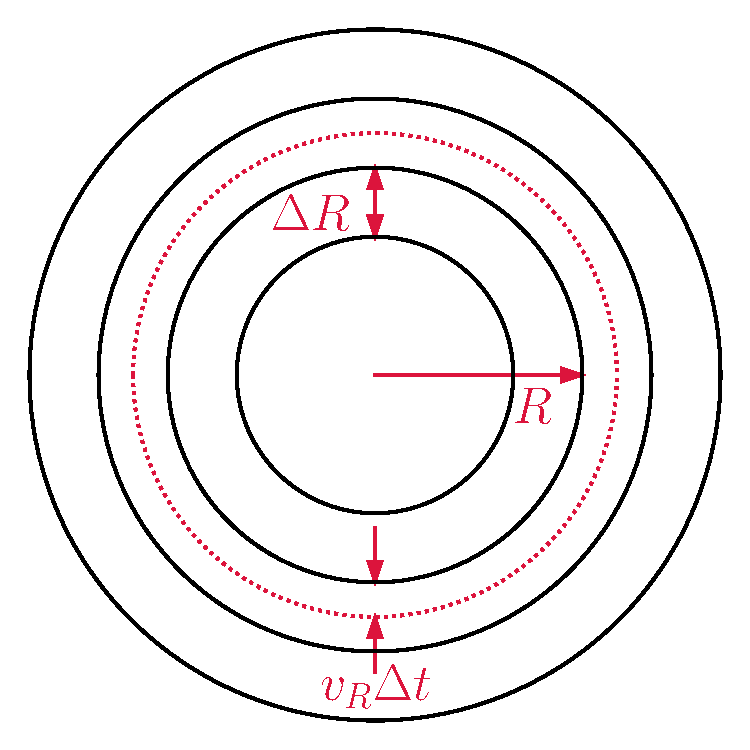
\includegraphics[scale = 0.5]{chapter7/schematic.pdf}
\caption{
A schematic of our derivation of the flow coefficients~$\mu_\flow$
and~$\gamma_\flow$.}
\label{outflows:fig:coefficients-schematic}
\end{figure}

In this Appendix, we present a detailed derivation of the radial gas flow
coefficients~$\gamma_\flow$ and~$\mu_\flow$ given by equations
\refp{outflows:eq:gamma-flow-general} and~\refp{outflows:eq:mu-flow-general}
in~\S~\ref{outflows:sec:gce:onezone}.
We begin by considering a narrow ring embedded in the Milky Way disk spanning
the radial range [$R$, $R + \Delta R$) where the evolution is discretized into
differential timesteps of size~$\Delta t$.
Fig.~\ref{outflows:fig:coefficients-schematic} shows a schematic of this
spatial configuration.
We first derive an expression for the flow rates under this approximation and
subsequently demonstrate that our expressions for~$\gamma_\flow$
and~$\mu_\flow$ arise in the limit that~$\Delta R$,~$\Delta t \rightarrow 0$.
We focus on a derivation of~$\mu_\flow$ as the derivation of~$\gamma_\flow$
follows similarly.
\par
Because radial flows are generally directed inward (see discussion
in~\S~\ref{outflows:sec:gce:onezone}), an annulus at a radius~$R$ tends to
experience a net gain of material from its neighbor at~$R + \Delta R$ and a net
loss to its neighbor at~$R - \Delta R$.
The relative values of these two terms then determines if radial gas flows are
an overall net source or sink.
For notational convenience, we briefly diverge from conventional notation and
define an inward gas velocity to have positive sign (i.e.,~$v_g > 0$) and
simply apply a~$v_g \rightarrow -v_g$ transformation at the end.
\par
We assume that the ISM is chemically homogeneous and with a uniform density
within each annulus, an approximation which should be valid since we eventually
take the limit as~$\Delta R \rightarrow 0$.
Since this derivation is motivated by treating each annulus as a one-zone GCE
model, there is no spatial information available in our primary use-case anyway.
Although the ISM should have a distribution of radial velocities from different
fluid elements, we also assume that all of the gas is moving at the same
velocity~$v_g$.
In this limit, an annulus whose inner radius is~$R$ will lose all of the gas
between~$R$ and~$R + v_g \Delta t$.
The mass that migrates inward can then be expressed according to the area
fraction~$a$ given by
\begin{equation}
a = \frac{
	2 R v_g \Delta t + v_g^2 \Delta t^2
}{
	2 R \Delta R + \Delta R^2
}.
\label{outflows:eq:area-frac-def}
\end{equation}
Simultaneously, material will be gained from the next ring outward, which spans
radii [$R + \Delta R$, $R + 2\Delta R$).
The net flow rate of some element~$x$ can then be expressed as the difference
of these two source and sink terms:
\begin{equation}\begin{split}
\dot{M}_{x,\flow} &= \dot{M}_{x,\flow,\text{in}} -
\dot{M}_{x,\flow,\text{out}}
\\
&= Z_x(R + \Delta R) M_g(R + \Delta R) \frac{a(R + \Delta R)}{\Delta t} -
Z_x(R) M_g(R) \frac{a(R)}{\Delta t}
\\
&= Z_x(R) M_g(R) \frac{a(R)}{\Delta t}
\left[
\frac{Z_x(R + \Delta R) M_g(R + \Delta R) a(R + \Delta R)}{Z_x(R) M_g(R) a(R)}
- 1\right].
\label{outflows:eq:flowin-minus-flowout}
\end{split}\end{equation}
This expression accounts for non-uniform radial velocity fields by simply
letting~$v_g$ vary with~$R$, and the effects are tracked automatically
through~$a(R)$.
Regardless of the functional forms of~$Z_x(R)$ and~$M_g(R)$, they can be
expressed as Taylor series, along with~$a$:
\begin{subequations}\begin{align}
Z_x(R + \Delta R) &= Z_x(R) + \sum_{i = 1}^\infty
\frac{\partial^i Z_x}{\partial R^i} \Delta R^i
\\
M_g(R + \Delta R) &= M_g(R) + \sum_{i = 1}^\infty
\frac{\partial^i M_g}{\partial R^i} \Delta R^i
\\
a(R + \Delta R) &= a(R) + \sum_{i = 1}^\infty
\frac{\partial^i a}{\partial R^i} \Delta R^i.
\end{align}\end{subequations}
Although it is straightforward to evaluate~$a(R + \Delta R)$ with
equation~\refp{outflows:eq:area-frac-def}, it is notationally useful for this
derivation to express it as a Taylor expansion.
\par
We stop noting~$Z_x$,~$M_g$, and~$a$ as functions of radius hereafter as they
are all evaluated at~$R$ as opposed to~$R + \Delta R$.
The flow rate~$\dot{M}_{x,\flow}$ then becomes
\begin{equation}
\dot{M}_{x,\flow} = Z_x M_g
\frac{2 R v_g + v_g^2 \Delta t}{2 R \Delta R + \Delta R^2} \Gamma,
\end{equation}
where we have plugged in equation~\refp{outflows:eq:area-frac-def}
for~$a / \Delta t$, and~$\Gamma$ is defined as
\begin{equation}\begin{split}
\Gamma &\equiv
\left(1 + \frac{1}{Z_x}
\sum_{i = 1}^\infty \frac{\partial^i Z_x}{\partial R^i} \Delta R^i\right)
\left(1 + \frac{1}{M_g}
\sum_{i = 1}^\infty \frac{\partial^i M_g}{\partial R^i} \Delta R^i\right)
\Bigg(1 +
\\
&\qquad
\frac{1}{a}
\sum_{i = 1}^\infty \frac{\partial^i a}{\partial R^i} \Delta R^i\Bigg) - 1.
\end{split}\end{equation}
Taking the limit of the flow rate as~$\Delta R \rightarrow 0$ requires
L'H\^opital's rule as both $2 R \Delta R + \Delta R^2 \rightarrow 0$
and~$\Gamma \rightarrow 0$.
We therefore differentiate both of them with respect to~$\Delta R$:
\begin{equation}\begin{split}
\frac{\partial \Gamma}{\partial \Delta R} &=
\left(\frac{1}{Z_x} \sum_{i = 1}^\infty i
\frac{\partial^i Z_x}{\partial R^i} \Delta R^{i - 1}\right)
\left(1 + \frac{1}{M_g}
\sum_{i = 1}^\infty \frac{\partial^i M_g}{\partial R^i} \Delta R^i\right)
\\
&\quad
\left(1 + \frac{1}{a}
\sum_{i = 1}^\infty \frac{\partial^i a}{\partial R^i} \Delta R^i\right) +
\\
&\quad
\left(1 + \frac{1}{Z_x}
\sum_{i = 1}^\infty \frac{\partial^i Z_x}{\partial R^i} \Delta R^i\right)
\left(\frac{1}{M_g} \sum_{i = 1}^\infty i
\frac{\partial^i M_g}{\partial R^i} \Delta R^{i - 1}\right)
\\
&\quad
\left(1 + \frac{1}{a}
\sum_{i = 1}^\infty \frac{\partial^i a}{\partial R^i} \Delta R^i\right) +
\\
&\quad
\left(1 + \frac{1}{Z_x}
\sum_{i = 1}^\infty \frac{\partial^i Z_x}{\partial R^i} \Delta R^i\right)
\left(1 + \frac{1}{M_g}
\sum_{i = 1}^\infty \frac{\partial^i M_g}{\partial R^i} \Delta R^i\right)
\\
&\quad
\left(\frac{1}{a} \sum_{i = 1}^\infty i \frac{\partial^i a}{\partial R^i}
\Delta R^{i - 1}\right).
\end{split}\end{equation}
Despite the complicated nature of this expression, the limit as
$\Delta R \rightarrow 0$ results in all terms except those
with~$\Delta R^{i - 1}$ paired with~$i = 1$ to drop out.
In the denominator, differentiation yields
$2 R \Delta R + \Delta R^2 \rightarrow 2R + \Delta R$, and we arrive at the
following expression for the flow rate:
\begin{equation}
\dot{M}_{x,\flow} = Z_x M_g \frac{2 R v_g + v_g^2 \Delta t}{2R} \left[
\frac{1}{Z_x} \frac{\partial Z_x}{\partial R} +
\frac{1}{M_g} \frac{\partial M_g}{\partial R} +
\lim_{\Delta R \rightarrow 0} \frac{1}{a} \frac{\partial a}{\partial R}
\right].
\label{outflows:eq:mdot-flow-limit}
\end{equation}
We leave the limit on~$(1 / a) \partial a / \partial R$ for now as it has a
uniquely defined solution given equation~\refp{outflows:eq:area-frac-def}, and
from there it follows that
\begin{equation}
\lim_{\Delta R, \Delta t \rightarrow 0} \frac{1}{a}
\frac{\partial a}{\partial R} = \frac{1}{v_g} \frac{\partial v_g}{\partial R}.
\end{equation}
\par
We now make a handful of final substitutions.
First, we plug in~$\tau_\star \equiv M_g / \dot{M}_\star$ outside of the square
brackets in equation~\refp{outflows:eq:mdot-flow-limit} so that the flow rate
is expressed in terms of the SFR as in~\S~\ref{outflows:sec:gce:onezone}.
Second, it is straightforward to show that
\begin{equation}
\frac{1}{M_g} \frac{\partial M_g}{\partial R} =
\frac{1}{R} + \frac{1}{\Sigma_g} \frac{\partial \Sigma_g}{\partial R},
\end{equation}
and in most cases it will be a more attractive option to specify the surface
density~$\Sigma_g$ as an input parameter as opposed the mass profile.
We also apply the~$v_g \rightarrow -v_g$ transformation to realign with
conventional notation where inward velocities have negative sign.
We also cancel the~$v_g^2 \Delta t$ term as a consequence of the limit
that~$\Delta t \rightarrow 0$.
Combining terms and applying the identity~$d \ln x = dx / x$, we arrive at the
following expression for the metal flow rate:
\begin{equation}
\dot{M}_{x,\flow} = -Z_x \dot{M}_\star \tau_\star v_g
\left[
\frac{1}{R} +
\frac{\partial \ln \Sigma_g}{\partial R} +
\frac{\partial \ln v_g}{\partial R} +
\frac{\partial \ln Z_x}{\partial R}
\right].
\label{outflows:eq:mdot-element-result}
\end{equation}
As mentioned at the beginning of this Appendix, an expression for the gas flow
rate~$\dot{M}_g$ follows similarly follows a similar derivation.
The only difference is that no consideration for the metal mass fraction
$Z_x$ is required.
Its form can also be easily deduced by simply setting~$Z_x = 1$ at all radii:
\begin{equation}
\dot{M}_{g,\flow} = -\dot{M}_\star \tau_\star v_g \left[
\frac{1}{R} +
\frac{\partial \ln \Sigma_g}{\partial R} +
\frac{\partial \ln v_g}{\partial R}
\right].
\label{outflows:eq:mdot-gas-result}
\end{equation}
At this point, the proper forms of the flow coefficients~$\gamma_\flow$
and~$\mu_\flow$ given by equations~\refp{outflows:eq:gamma-flow-general}
and~\refp{outflows:eq:mu-flow-general} are now clear.
\par
The same derivation applies in the limit that these rates are computed for a
single timestep.
Since we have taken the limit as~$\Delta t \rightarrow 0$, we can therefore
assert without loss of generality that the quantities in equations
\refp{outflows:eq:mdot-element-result} and~\refp{outflows:eq:mdot-gas-result}
may be arbitrary, continuous functions of time.
However, as we demonstrate throughout chapter~\ref{outflows}, holding them
fixed in time still leads to enlightening analytic solutions.

\end{document}

